\section{Resultados}
\label{sec:resultados}

Se presentan primero los parámetros calibrados (módulo microbiano contra los controles; núcleo larvario contra las tasas netas) y luego la validación por descomposición de fuentes.

\subsection{Calibración del módulo microbiano con los controles de alimento solo}

Las curvas de control (alimento sin larvas) aislaron la componente microbiana. El ajuste de $k_{\mathrm{ref}}$ e $Y_{CO_2}$ por mínimos cuadrados dio valores consistentes entre dietas: $k_{\mathrm{ref}} = 0.282$ d$^{-1}$ e $Y_{CO_2} = 1.39$ para D1, y $k_{\mathrm{ref}} = 0.290$ d$^{-1}$ e $Y_{CO_2} = 1.13$ para D4. Con el estado de biomasa microbiana, el módulo reproduce tanto la magnitud como la tendencia creciente de las tasas de control ($R^2 = 0.968$ y $0.982$; RMSE de 1.0 y 1.5 ppm/min para D1 y D4; Figuras \ref{fig:valD1} y \ref{fig:valD4}): el aumento sostenido de las tasas de control corresponde al crecimiento de la biomasa microbiana sobre el sustrato.

\subsection{Ajuste conjunto del núcleo larvario}

El ajuste conjunto sobre las tasas netas (tratamiento menos control del mismo día, promedio de tres cierres consecutivos) dio una biomasa inicial $B_0 = 0.0735$ mg/larva, del orden de la biomasa de una larva neonata (decenas de \textmu g); un factor de calidad de dieta $f = 0.698$ para D4 (D1 = 1, dieta de referencia de \textcite{eriksenDynamicModellingFeed2022}); tiempos centrales de prepupa $t_p = 16.4$ d para D1 y $t_p = 12.1$ d para D4; y un ancho de transición $w_p = 0.36$ d, es decir, un cese de la alimentación que ocurre en torno a un día. El ajuste usó cuatro grados de libertad frente a cuatro puntos no saturados (uno en D1 y tres en D4) más tres cotas inferiores; el $R^2$ reportado debe leerse con ese tamaño muestral. Los parámetros cinéticos del núcleo DEB se mantuvieron fijos en los valores de la literatura (Cuadro \ref{tab:parametros}).

\subsection{Validación por descomposición de fuentes}

El Cuadro \ref{tab:tasas} resume la comparación y las Figuras \ref{fig:valD1} y \ref{fig:valD4} muestran las curvas del modelo contra las mediciones.

Para D4, la componente larvaria reproduce las tres tasas netas no saturadas con $R^2 = 0.981$ y RMSE de 5.2 ppm/min (89.0 frente a 88.6 el día 9; 21.3 frente a 21.5 el día 13; 9.0 frente a 0.0 el día 17), y satisface la cota inferior del día 11 (164.7 frente a 165.4 ppm/min, $-0.4$ \%). El suelo de mantenimiento en prepupa (9.0 ppm/min el día 17) queda cercano a la tasa de larvas en ayuno medida ese mismo día (14.3 ppm/min), lo que respalda el anclaje de $m_{\mathrm{suelo}}$: la medición de ayuno proviene de un tratamiento independiente (larvas sin alimento) y no entró en la calibración.

Para D1, el modelo reproduce la forma de la trayectoria pero no todos los puntos: satisface la cota inferior del día 9 (267.9 frente a 267.8 ppm/min, $+0.0$ \%) y queda a un 10 \% del único punto no saturado (día 13: 92.2 frente a 102.8 ppm/min), pero no alcanza la cota inferior del día 11 (92.2 frente a 124.3 ppm/min, $-25.9$ \%). En el modelo la causa es estructural: con 75~g de materia seca para 700 larvas ($\approx 107$~mg de sustrato por larva, en el rango de ración por larva del modelo de referencia), las larvas agotan la fracción degradable del lecho hacia el día 10 y la tasa larvaria cae a la respiración de mantenimiento ($\approx 92$~ppm/min) antes de que opere el interruptor de prepupa ($t_p = 16.4$~d, ya al final de la ventana experimental). Es decir, para D1 el colapso de emisiones observado entre los días 9 y 11 se atribuye al agotamiento del alimento y no a la transición a prepupa, y la subestimación del día 11 indica que el agotamiento real fue más gradual que el del modelo, compatible con un lecho heterogéneo que la formulación de parámetros concentrados no representa. La tasa del día 11 proviene además del cierre con el ajuste lineal de menor calidad ($R^2 = 0.76$), por lo que la discrepancia real puede ser aún mayor; se retoma en la discusión.

Cabe notar que el RMSE de la componente larvaria en D4 (5.2 ppm/min) es del orden de la incertidumbre instrumental estimada para esas tasas (6 a 10 ppm/min, sec. \ref{sec:incertidumbre}), de modo que la componente larvaria reproduce las tasas netas de D4 dentro de la incertidumbre experimental; las discrepancias restantes (la cota inferior del día 11 de D1, que el modelo no alcanza, y el apagado del término microbiano en el tratamiento de D1 cuando las larvas agotan el sustrato) son estructurales y no instrumentales; se retoman en la discusión.

La componente total (larvaria más microbiana) reproduce el orden de magnitud y la forma temporal de las tasas de tratamiento en ambas dietas, incluidos el pico previo al colapso y el colapso mismo, que el modelo atribuye al agotamiento del sustrato en D1 y a la transición a prepupa en D4.

\begin{table}[htbp]
\centering
\small
\caption{Tasas de CO$_2$ observadas y modeladas por dieta y día de medición, en ppm/min: componente microbiana frente a controles de alimento solo; componente larvaria frente a la tasa neta (tratamiento menos control); total frente a tratamiento. ($^{*}$) cierre saturado: la tasa observada es una cota inferior (ver texto). En el tratamiento de D1 el total modelado de los días 11 y 13 es solo la componente larvaria: las larvas agotan la fracción degradable del sustrato hacia el día 10 y el término microbiano se apaga (sec. 2.2.2).}
\label{tab:tasas}
\begin{tabular}{ll rrr rr rr}
\toprule
Dieta & Día & \multicolumn{2}{c}{Microbiana} & \multicolumn{2}{c}{Larvaria (neta)} & \multicolumn{2}{c}{Total} \\
\cmidrule(lr){3-4} \cmidrule(lr){5-6} \cmidrule(lr){7-8}
 & & obs. & mod. & obs. & mod. & obs. & mod. \\
\midrule
D1 & 9  & 26.5 & 27.4 & 267.8$^{*}$ & 267.9 & 294.3 & 280.8 \\
   & 11 & 34.8 & 33.4 & 124.3$^{*}$ & 92.2 & 159.1 & 92.2 \\
   & 13 & 40.2 & 40.8 & 102.8 & 92.2 & 143.0 & 92.2 \\
\midrule
D4 & 9  & 25.8 & 23.6 & 88.6 & 89.0 & 114.4 & 112.4 \\
   & 11 & 27.2 & 28.9 & 165.4$^{*}$ & 164.7 & 192.5 & 192.3 \\
   & 13 & 34.6 & 35.5 & 21.5 & 21.3 & 56.1 & 51.5 \\
   & 17 & 54.1 & 53.5 & 0.0 & 9.0 & 40.0 & 49.2 \\
\bottomrule
\end{tabular}
\end{table}

\begin{figure}[htbp]
\centering
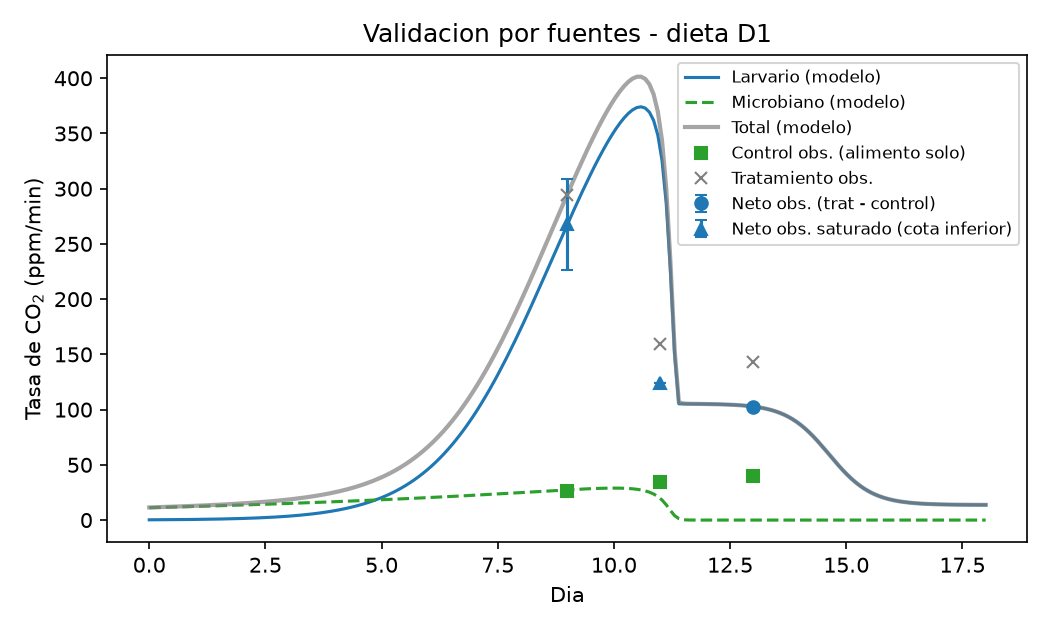
\includegraphics[width=0.85\textwidth]{figuras/validacion_co2_D1.png}
\caption{Validación por descomposición de fuentes, dieta D1 (alimento estándar). Curvas: componentes larvaria y microbiana y total del modelo para el régimen de carga única. Puntos: controles de alimento solo (cuadrados), tratamiento (x) y tasa neta tratamiento menos control (círculos; triángulos: cierres saturados, es decir cotas inferiores, con el rango entre cierres).}
\label{fig:valD1}
\end{figure}

\begin{figure}[htbp]
\centering
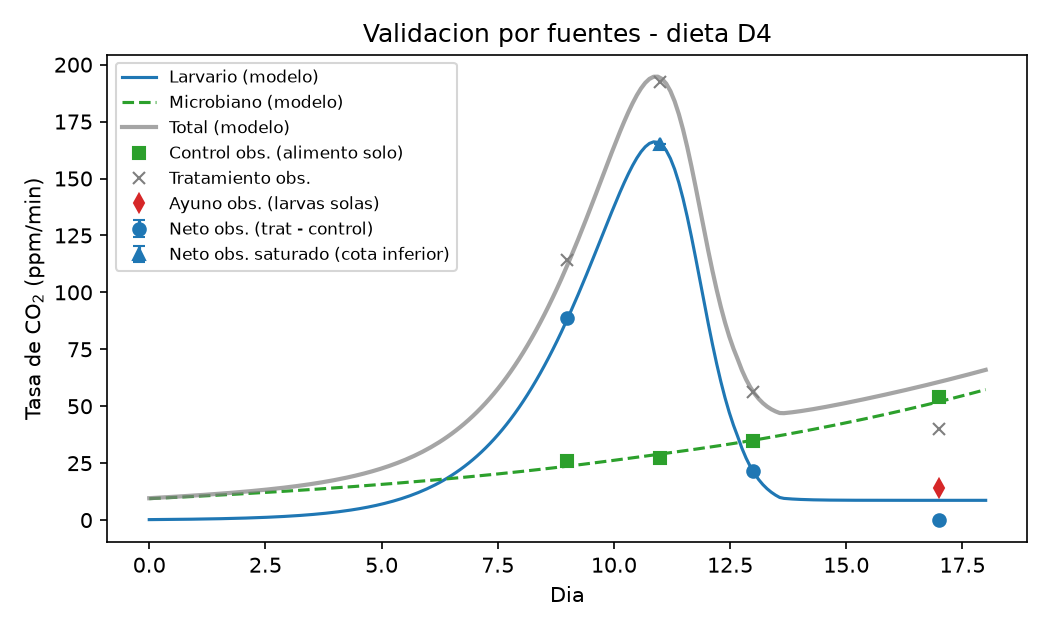
\includegraphics[width=0.85\textwidth]{figuras/validacion_co2_D4.png}
\caption{Validación por descomposición de fuentes, dieta D4 (residuos agroindustriales de frutas). Simbología como en la Figura \ref{fig:valD1}; el diamante es la tasa de larvas en ayuno medida el día 17.}
\label{fig:valD4}
\end{figure}

\paragraph{Nota sobre el CH$_4$.}
El canal de CH$_4$ (verificado en 0--10~\% en volumen) registró acumulaciones claramente medibles (pendientes de 300 a 3200~ppm/min, con $R^2 \geq 0.9$ en la mayoría de los cierres), pero sus dinámicas no fueron compatibles con la estructura del modelo: los controles de alimento solo decrecieron a lo largo del ciclo (de 1633 a 560~ppm/min en D1) mientras la degradación microbiana crece, los tratamientos no se separaron de forma consistente de sus controles (el día 9 midieron menos CH$_4$ que el control en ambas dietas) y aparecieron picos tardíos aislados (D4, día 17). Este patrón es atribuible a respuesta parcial del canal de CH$_4$ a volátiles de la fermentación del sustrato (etanol y otros compuestos orgánicos volátiles), y no a metanogénesis sola; por ello el término $\xi(\theta_s)$ del modelo se mantiene como indicador cualitativo de microambientes anóxicos y las lecturas de CH$_4$ se excluyeron de la validación cuantitativa; se retoma en la discusión.

\subsection{Análisis de sensibilidad}
Para evaluar cuánto dependen las conclusiones de los parámetros tomados de la literatura y del número aproximado de larvas, se recalibraron $B_0$, $f$, $t_p$ y $w_p$ perturbando uno a la vez $m$, $a_{\max}$ y $N$ en $\pm 20$~\% (Cuadro~\ref{tab:sensibilidad}). El ajuste es robusto al mantenimiento ($m$ $\pm 20$~\%: $R^2 \approx 0.98$ en D4, RMSE de 5.3 a 5.6 ppm/min), pero sensible a $a_{\max}$ y $N$: con $\pm 20$~\% el $R^2$ de D4 cae a $-2.44$ y $0.09$ ($a_{\max}$) y a $0.84$ y $0.93$ ($N$), y algunas cotas inferiores adicionales dejan de satisfacerse. La cota del día 11 de D1 queda incumplida en el caso base y en todos los escenarios de perturbación, lo que confirma su origen estructural (el agotamiento del sustrato en D1) y no un accidente de la calibración. Es decir, las tasas de gas sí restringen la combinación de parámetros: los valores cinéticos del núcleo DEB no son intercambiables, las conclusiones son condicionales a esos valores de la literatura y la sensibilidad cuantificada define la magnitud del riesgo, lo que refuerza la necesidad de una validación directa de biomasa que los fije de forma independiente.

\begin{table}[htbp]
\centering
\caption{Análisis de sensibilidad uno a la vez ($\pm 20$~\%) sobre los parámetros fijos $m$, $a_{\mathrm{máx}}$ y $N$, recalibrando $B_0$, $f$, $t_p$ y $w_p$ en cada caso. RMSE en ppm/min sobre los puntos no saturados (en D1, un solo punto); cotas D1/D4: margen porcentual mínimo sobre las cotas inferiores de los cierres saturados de cada dieta (negativo: cota violada).}
\label{tab:sensibilidad}
\begin{tabular}{lrrrrrrr}
\toprule
Perturbación & $B_0$ (mg) & $f$ (D4) & $R^2$ (D4) & RMSE (D4) & RMSE (D1) & cota D1 (\%) & cota D4 (\%) \\
\midrule
Base            & 0.0735 & 0.698 &  0.981 &  5.2 & 10.6 & $-25.9$ &  $-0.4$ \\
$m$ $-20$~\%    & 0.0656 & 0.705 &  0.980 &  5.3 & 10.7 & $-25.9$ &  $-1.9$ \\
$m$ $+20$~\%    & 0.0813 & 0.693 &  0.978 &  5.6 & 16.0 & $-25.8$ &    1.4  \\
$a_{\max}$ $-20$~\% & 0.278 & 0.730 & $-2.44$ & 69.9 &  9.9 & $-65.3$ & $-46.0$ \\
$a_{\max}$ $+20$~\% & 0.0136 & 0.722 & 0.086 & 36.1 & 11.9 & $-24.2$ & $-64.3$ \\
$N$ $-20$~\%    & 0.0924 & 0.711 &  0.840 & 15.1 & 10.5 & $-50.0$ &   21.6  \\
$N$ $+20$~\%    & 0.0515 & 0.707 &  0.933 &  9.8 & 10.8 & $-26.0$ & $-16.1$ \\
\bottomrule
\end{tabular}
\end{table}
